%%!TEX root = ./UserManual.tex
\chapter{Visualization}
\label{chap:visualizer}


\section{Visualization files}

Visualization files (\texttt{*\_vis.json}) are only produced by the simulator when working with a population generated from a geographical distribution, as otherwise there's no data to determine the locations of clusters on a map.

\section{The Visualizer}

\begin{figure}[t]
	\centering
	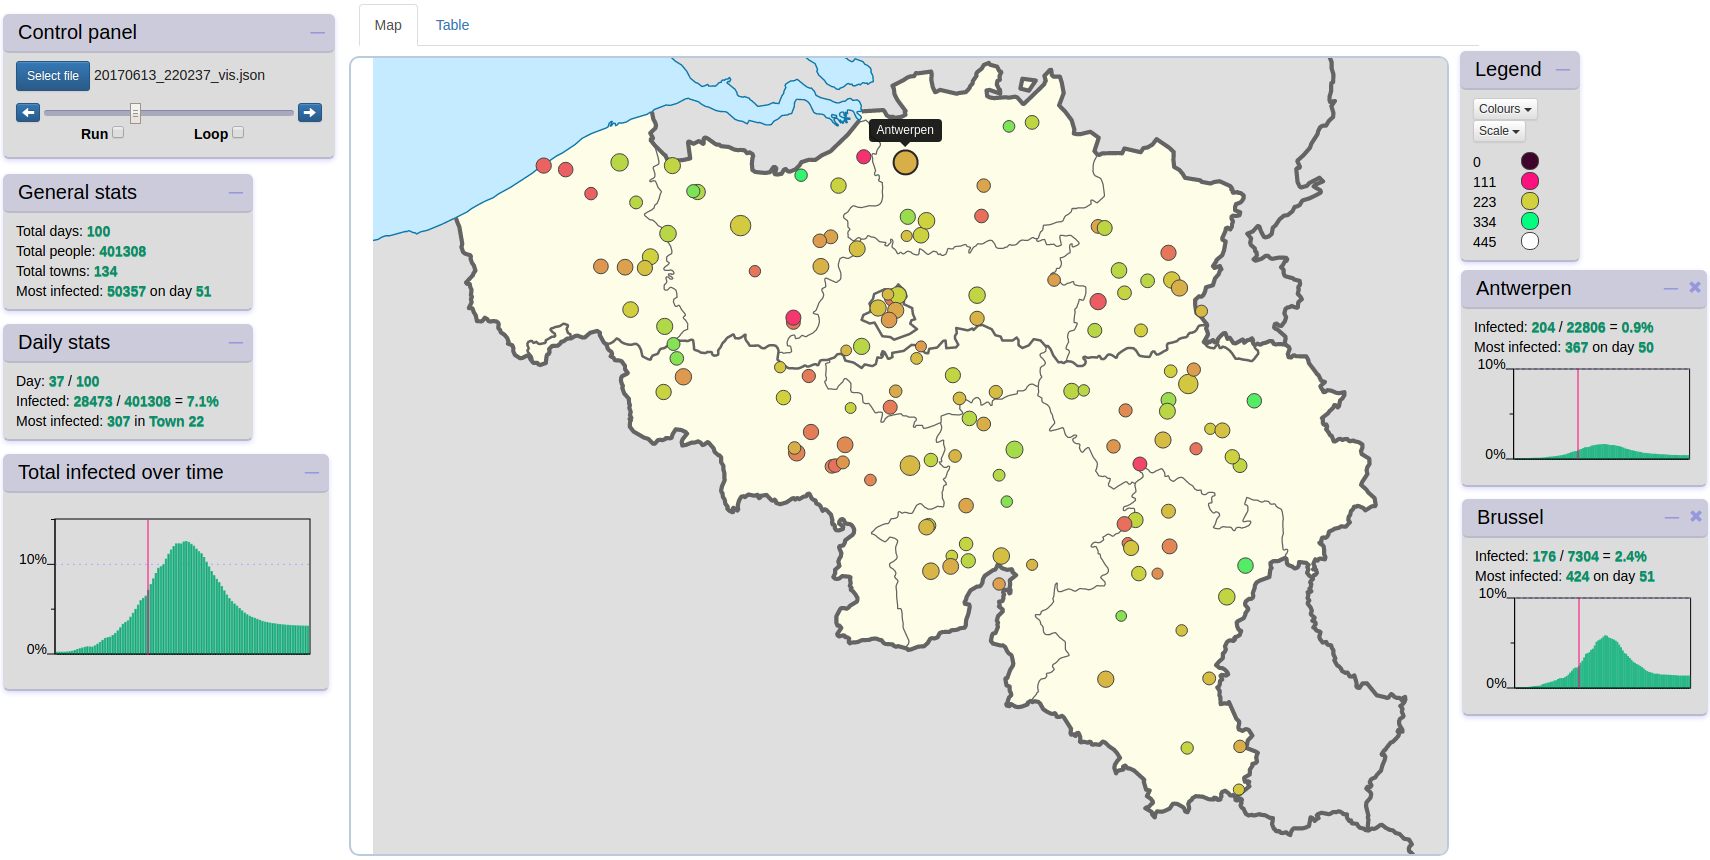
\includegraphics[width=\textwidth]{images/visualizer.png}
	\caption{A visualization showing the map view and all panels.}
\end{figure}

The visualizer is a JavaScript-based browser application. It is included in the Stride distribution in \texttt{src/main/resources/html/main.html}, or it can be accessed from \url{https://flu-plus-plus.github.io/visualizer/main.html}.


\subsection{Loading a file}

To load a visualization file simply click the "Select file" button on the control panel. Selecting a file automatically analyses the data and starts the visualization.

\subsection{Controlling time}

On the control panel, use the left and right buttons to step through the timeline one day at a time, or use the slider for greater control over the currently visualized day.

The checkbox marked ``{Run}'' will cause the visualizer to automatically step through the timeline one day at a time until it reaches the end. If the box marked ``{Loop}'' is checked the visualizer will instead jump back to the first day and continue running.


\subsection{The map view}

After loading a valid file, the map view will automatically plot the data on an appropriate map. By default the visualizer will fall back to a high-resolution map of the entire world. If you wish to extend the visualizer to use more appropriate map images for plotting, consult \texttt{Map.js}.

Each location is represented by a circle on the map with several attributes:

\begin{compactitem}

\item \textbf{Size:} The size of the circle corresponds to the number of inhabitants in that location.
\item \textbf{Colour:} The colour of the circle corresponds to the amount of infected inhabitants in the location. For more info see the section on the legend panel.
\item \textbf{Hover:} Hovering over a circle will display the name of the location it represents.
\item \textbf{Click:} Clicking a circle will open a new location specific panel.

\end{compactitem}

\subsection{The legend panel}

The legend panel shows and controls the map's colour coding.

The selector labeled ``Colours'' allows you to choose the colour scheme employed by the map view. Options include \textit{Monochrome}, \textit{Heat map} and \textit{Rainbow}. If you wish to add more possible colour schemes, consult \texttt{Colour.js}.

The selector labeled ``Scale'' allows you to choose what the colours represent:
\begin{compactitem}
	
	\item \textbf{Count:} The colour of a circle corresponds to the absolute quantity of infected.
	\item \textbf{Percentage:} The colour of a circle corresponds to the percentage of infected.
	
\end{compactitem}

\subsection{The table view}

The table view is an alternate visualization option, showing the same data as the map except in a text-based representation. It is accessed by clicking the ``Table'' tab at the top of the page.

The columns are as follows:

\begin{compactitem}
	
	\item \textbf{Name:} The name of the location. Clicking this will open a location specific panel.
	\item \textbf{Inhabitants:} The total number of inhabitants in the location.
	\item \textbf{Current infected:} The absolute and relative quantity of infected in the location.
	\item \textbf{Most infected:} The highest number of infected in that location, and the day on which it happened. Clicking the day will automatically set the timeline to that day.
	
\end{compactitem}


\subsection{The panels}

Panels can be moved, minimized, and some can even be deleted.

The control panel and legend panel have already been discussed.

\subsubsection{General stats panel}
This panel holds information that is constant for the entire file.
\begin{compactitem}	
	\item \textbf{Total days:} The total number of logged days.
	\item \textbf{Total people:} The total number of inhabitants across all locations.
	\item \textbf{Most infected:} The highest total number of infected of all time, and the day on which it happened. Clicking the day will automatically set the timeline to that day.
\end{compactitem}


\subsubsection{Daily stats panel}
This panel holds information that changes between days.
\begin{compactitem}	
	\item \textbf{Day:} The currently selected day, compared to the total number of days.
	\item \textbf{Infected:} The total number of infected across all locations, compared to the total number of people.
	\item \textbf{Most infected:} The highest number of infected in a single location, and the location on which it happened. Clicking the location name will open a location specific panel.
\end{compactitem}

\subsubsection{Total infected over time panel}
This panel shows a graph representing the combined percentage of infected over the entire logged length of time.

\subsubsection{Location specific panels}
These panels show data specific to a given location.
\begin{compactitem}	
	\item \textbf{Infected:} The number of infected, compared to the number of inhabitants.
	\item \textbf{Most infected:} The highest number of infected of all time, and the day on which it happened. Clicking the day will automatically set the timeline to that day.
	\item A graph showing the percentage of infected in the location over time.
\end{compactitem}